% performance / speed(efficiency) / 

% \COMMENT{add one more figure to visualize the methods and exp results}
% \haonan{more quali results (policy is smooth, rollout, perturbation)}



\vspace{-7pt}
\section{Experiments}
\vspace{-3pt}


% \begin{figure*}[ht!]
% \centering

% \newlength{\subfigw}
% \newlength{\colgap}
% \newlength{\rowgap}
% \setlength{\subfigw}{0.31\textwidth}
% \setlength{\colgap}{0.015\textwidth}
% \setlength{\rowgap}{3pt}

% \captionsetup[subfigure]{
%   justification=centering,
%   singlelinecheck=true,
%   font=footnotesize,
%   labelformat=empty,
%   skip=2pt
% }

% \begin{subfigure}[t]{\subfigw}
%   \centering
%   \includegraphics[width=\linewidth]{images/pick-cube-setup-1.pdf}

%   \vspace{\rowgap}

%   \includegraphics[width=\linewidth]{images/pick-cube-distribution.pdf}
%   \caption{\pickcube.}
%   \label{fig:pick-cube-distribution}
% \end{subfigure}
% \hspace{\colgap}
% \begin{subfigure}[t]{\subfigw}
%   \centering
%   \includegraphics[width=\linewidth]{images/clean-table-setup-1.pdf}

%   % \vspace{\rowgap}

%   \includegraphics[width=\linewidth]{images/clean-table-distribution.pdf}
%   \caption{\cleantable.}
%   \label{fig:clean-table-distribution}
% \end{subfigure}
% \hspace{\colgap}
% \begin{subfigure}[t]{\subfigw}
%   \centering
%   \includegraphics[width=\linewidth]{images/speeding-cup-setup-1.png}

%   \vspace{\rowgap}

%   \includegraphics[width=\linewidth]{images/speeding-cup-distribution.pdf}
%   \caption{\stackunstack.}
%   \label{fig:stack-unstack-distribution}
% \end{subfigure}

% \vspace{-5pt}

% \caption{\textbf{Overview of the real-world tasks.} Top row: Task setups for \pickcube, \cleantable, and \stackunstack. Bottom row: Corresponding object initialization distributions and workspace sizes. These tasks vary in precision requirements, horizon length, and object interactions, highlighting the challenges of fast manipulation due to tight precision requirements, long task horizons, and complex object interactions.}
% \label{fig:real-world-setup}
% \vspace{-10pt}
% \end{figure*}
% \vspace{-10pt}
We integrate \our with two imitation-learning backbones:
(i) Diffusion Policy~\cite{dp}, denoted as Diff.+BSP, and
(ii) Action Chunking with Transformers (ACT)~\cite{act}, denoted as Reg.+BSP.
We evaluate \our along two main metrics: 
\textbf{(1)} \textit{\textbf{success rate}}, measured across a diverse set of tasks, and 
\textbf{(2)} \textit{\textbf{average completion time}}, measured by the mean task completion time across successful rollouts.
%
To this end, we evaluate our method against baseline policies on three real-world tasks that span diverse manipulation challenges: \pickcube, which requires precise object manipulation; \cleantable, which involves long-horizon tabletop rearrangement; and \stackunstack, which emphasizes bimanual, contact-rich interaction. We also benchmark \our in simulation environments on \textit{Push-T}~\cite{florence2022implicit,dp}, \textit{RoboMimic}~\cite{robomimic2021} and \textit{RoboCasa}~\cite{nasiriany2024robocasa}.



% \begin{figure*}
%     \centering
%     % \includegraphics[width=1\linewidth]{images/visualize-tasks.pdf}
%     \includegraphics[width=1\linewidth]{images/visualize-tasks-compact.pdf}
%     \caption{\textbf{Overview of the real-world tasks.} 
%     For each task, we show key frames from left to right, followed by the corresponding distribution of evaluation configurations. The tasks vary in precision requirements, horizon length, and object interactions, highlighting the challenges of fast manipulation.
%     }
%     \label{fig:real-world-setup}
%     \vspace{-15pt}
% \end{figure*}

    
\subsection{Real-world Experiments}
\label{sec:real-eval}
% The assets are in this link: https://drive.google.com/drive/folders/1QnWbk3FWm-cwOfLXTCbFc5YNjMjCm5iF?usp=share_link
% The editable version of the figure is in https://docs.google.com/presentation/d/1ehAGAqZKHBLXPHKu9jUsDhKJ6VEMvDzQ/edit?usp=share_link&ouid=108925265950662585086&rtpof=true&sd=true
\vspace{-5pt}

\noindent\textbf{Task setup.} In real-world experiments, we evaluate \our in the real world on three challenging tasks, as illustrated in Fig.~\ref{fig:real-world-setup}.
%
\noindent\textbf{\textit{1) \pickcube}.}
The robot is required to pick a cube and place it into a box on the table. We collect 200 demonstrations using cubes of four different colors. During both training and evaluation, only a single cube is present in the scene.
The cube has a side length of $3\,\mathrm{cm}$, requiring precise grasping and placement. \noindent\textbf{\textit{2) \cleantable}.}
This long-horizon manipulation task presents a significant challenge: the robot must clear a table by sequentially completing two subtasks: (i) picking two beverage cans and placing them into a designated plastic tray, and (ii) picking two empty bowls and placing them into a second tray, stacking the second bowl on top of the first. We collect 300 demonstrations for this task. 
%
\noindent\textbf{\textit{3) \stackunstack}.}
The robot must first construct a cup pyramid (2--1) from identical cups and then collapse it into a single nested stack using two arms.
Cups are randomly initialized within a clutter-free workspace. We collect 200 demonstrations and evaluate performance across diverse initial configurations.

All experiments use 6-DoF ARX5 robot arms. For \pickcube and \cleantable, we use a single third-person camera. For \stackunstack, we employ two wrist-mounted cameras in addition to a fixed third-person camera placed between the two arms.



\noindent\textbf{Baselines and Evaluation protocol.}
We compare \our against three classes of baselines:
\textbf{(1)} Diffusion policy~\cite{dp} and Regression policy~\cite{act}, which executes them at the original demonstration or control frequency. \textbf{(2)} Diffusion policy-$n$X and Regression policy-$n$X, which naively increase the execution frequency by a factor of $n$. This represents the most direct baseline for accelerating task execution. \textbf{(3)} DemoSpeedup~\cite{demospeedup}, which accelerates execution by temporally downsampling demonstration trajectories. 
%
For each real-world task, we evaluate all methods on 20 rollouts with distinct object layouts. To ensure fair comparisons, we first record a fixed set of test configurations using the camera system; for subsequent evaluations, the environment is reset by matching object placements to these recorded configurations. The distribution of all test configurations is shown in Fig.~\ref{fig:real-world-setup}. For grasping actions in \pickcube and \cleantable, we allow up to three grasp attempts as recovery. We report the average completion time, measured from the start at the home pose to the final gripper opening that marks task completion, averaged over all successful rollouts.
% \begin{figure*}[t!]
%   \centering
%   % --- Row 1: simulation tasks (full width) ---
%   % \includegraphics[width=0.98\textwidth]{images/sim-env.pdf}

%   % \vspace{-4pt}

%   % --- Row 2: simulation results (two half-width figures) ---
%   % \includegraphics[width=0.98\textwidth]{images/sim-results.pdf}\hfill
%   \includegraphics[width=1\linewidth]{images/bspline-speedup-subplots-no-annotations.pdf}
%   % \includegraphics[width=0.48\textwidth]{images/sim-results-dp.pdf}

%   \caption{\textbf{B-spline speedup ablations in the real world.} Results for both regression and diffusion backbones. Each entry reports the success rate and the average completion time. B-spline policy provides up to a $\mathbf{4.21\times}$ speedup over the base imitation-learning methods while achieving a higher success rate.}
%   \vspace{-10pt}
%   \label{fig:speed-ablation}
% \end{figure*}






\begin{figure*}[t]
    \centering
    % \includegraphics[width=1\linewidth]{images/smoothness.pdf}
    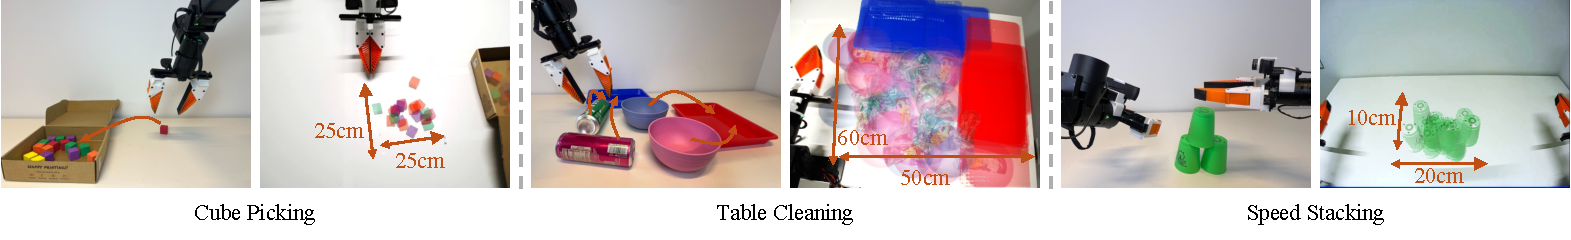
\includegraphics[width=1\linewidth]{images/real-world-task-setup.pdf}
    \vspace{-10pt}
    \caption{\textbf{Overview of the real-world tasks.} Task setups and corresponding object initialization distributions and workspace sizes for \pickcube, \cleantable, and \stackunstack.  These tasks vary in precision requirements, horizon length, and object interactions, highlighting the challenges of fast manipulation due to tight precision requirements, long task horizons, and complex object interactions.}

    \vspace{-10pt}

\label{fig:real-world-setup}
\end{figure*}



% \begin{table*}[h!]
%   \centering

%   % \renewcommand{\arraystretch}{1.15}
%   % \setlength{\tabcolsep}{6pt}
%   % \scriptsize     % CHAOQI: you can try this.
%   % \footnotesize
%   % \renewcommand{\arraystretch}{0.95}
%   % \setlength{\tabcolsep}{3pt}
%   \fontsize{7.4pt}{9pt}\selectfont
%   \renewcommand{\arraystretch}{0.98}
%   \setlength{\tabcolsep}{2pt}
  
%   % ---------------------- UP ----------------------
%   \subfloat{
%     \centering
%     \begin{tabular}{lc|c|ccc|cccc}
%       \toprule
%       Task & Metric &
%       DSP &
%       \makecell{Diffusion\\1X} &
%       \makecell{Diffusion\\2X} &
%       \makecell{Diffusion\\4X} &
%       \makecell{Diffusion +\\BSP 1X (ours)} &
%       \makecell{Diffusion +\\BSP 2X (ours)} &
%       \makecell{Diffusion +\\BSP 3X (ours)} &
%       \makecell{Diffusion +\\BSP 4X (ours)} \\
%       \midrule
%       \makecell{Cube \\ Picking} & \cellMetric &
%       \cellSRtime{18/20}{6.66s} &
%       \cellSRtime{19/20}{6.48s} &
%       \cellSRbold{20/20}{4.58s} &
%       \cellSRbold{20/20}{3.52s} &
%       \cellSRbold{20/20}{6.31s} &
%       \cellSRbold{20/20}{3.43s} &
%       \cellSRbold{20/20}{2.85s} &
%       \cellBothbold{20/20}{2.45s} \\
%       \midrule
%       \makecell{Table \\ Cleaning} & \cellMetric &
%       \cellSRtime{3/20}{49.47s} &
%       \cellSRtime{11/20}{41.40s} &
%       \cellSRbold{15/20}{28.87s} &
%       \cellSRtime{12/20}{23.31s} &
%       \cellSRbold{15/20}{36.97s} &
%       \cellSRtime{14/20}{20.81s} &
%       \cellTimebold{12/20}{17.30s} &
%       \cellSRtime{11/20}{18.05s} \\
%       \midrule
%       \makecell{Speed \\ Stacking} & \cellMetric &
%       \cellSRtime{3/20}{18.57s} &
%       \cellSRtime{14/20}{20.47s} &
%       \cellSRbold{15/20}{13.66s} &
%       \cellSRtime{9/20}{10.49s} &
%       \cellSRtime{14/20}{18.13s} &
%       \cellSRbold{15/20}{11.45s} &
%       \cellSRtime{11/20}{11.25s} &
%       \cellTimebold{7/20}{9.62s} \\
%       \bottomrule
%     \end{tabular}
%   }

%   \vspace{8pt}

%   % ---------------------- DOWN ----------------------
%   \subfloat{
%     \centering
%     \begin{tabular}{lc|c|ccc|cccc}
%       \toprule
%       Task & Metric &
%       DSP &
%       \makecell{Regression\\1X} &
%       \makecell{Regression\\2X} &
%       \makecell{Regression\\4X} &
%       \makecell{Regression +\\BSP 1X (ours)} &
%       \makecell{Regression +\\BSP 2X (ours)} &
%       \makecell{Regression +\\BSP 3X (ours)} &
%       \makecell{Regression +\\BSP 4X (ours)} \\
%       \midrule
%       \makecell{Cube \\ Picking} & \cellMetric &
%       \cellSRtime{18/20}{6.66s} &
%       \cellSRtime{18/20}{9.84s} &
%       \cellSRtime{15/20}{5.55s} &
%       \cellSRtime{19/20}{3.74s} &
%       \cellSRtime{19/20}{7.92s} &
%       \cellSRtime{19/20}{3.36s} &
%       \cellSRbold{20/20}{2.37s} &
%       \cellTimebold{19/20}{2.08s} \\
%       \midrule
%       \makecell{Table \\ Cleaning} & \cellMetric &
%       \cellSRtime{3/20}{49.47s} &
%       \cellSRtime{13/20}{49.70s} &
%       \cellSRtime{13/20}{34.48s} &
%       \cellSRtime{13/20}{23.57s} &
%       \cellSRbold{18/20}{38.47s} &
%       \cellSRbold{18/20}{19.11s} &
%       \cellSRtime{15/20}{13.34s} &
%       \cellTimebold{14/20}{11.80s} \\
%       \midrule
%       \makecell{Speed \\ Stacking} & \cellMetric &
%       \cellSRtime{3/20}{18.57s} &
%       \cellSRtime{8/20}{19.75s} &
%       \cellSRtime{4/20}{13.49s} &
%       \cellSRtime{8/20}{10.42s} &
%       \cellSRbold{16/20}{17.61s} &
%       \cellSRtime{13/20}{10.98s} &
%       \cellTimebold{7/20}{7.67s} &
%       \cellSRtime{0/20}{NA} \\
%       \bottomrule
%     \end{tabular}
%   }

% \caption{\todo \textbf{Real-world success rate and average completion time.}
% We report each method's success rate and average completion time on the real-world tasks. Completion time is averaged over successful trials only. For each task, we highlight the highest success rate and the shortest completion time. DSP denotes DemoSpeedup.}
% % \vspace{-20pt}
% \label{tab:act-dp-results}
% \end{table*}





% \begin{table*}[h!]
%   \centering

%   \fontsize{7.4pt}{9pt}\selectfont
%   \renewcommand{\arraystretch}{0.98}
%   \setlength{\tabcolsep}{2pt}
  
%   % ---------------------- UP ----------------------
%   \subfloat{
%     \centering
%     \begin{tabular}{lc|cc|cc|cc}
%       \toprule
%       Task & Metric &
%       \makecell{Diffusion\\1X} &
%       \makecell{Diffusion +\\BSP 1X (\textbf{ours})} &
%       \makecell{Diffusion\\2X} &
%       \makecell{Diffusion +\\BSP 2X (\textbf{ours})} &
%       \makecell{Diffusion\\4X} &
%       \makecell{Diffusion +\\BSP 4X (\textbf{ours})} \\
%       \midrule
%       \makecell{Cube \\ Picking} & \cellMetric &
%       \cellSRtime{19/20}{6.48s} &
%       \cellSRtime{\greenNum{20/20}}{\greenNum{6.31s}} &
%       \cellSRtime{20/20}{4.58s} &
%       \cellSRtime{\greenNum{20/20}}{\greenNum{3.43s}} &
%       \cellSRtime{20/20}{3.52s} &
%       \cellSRtime{\greenNum{20/20}}{\greenNum{2.45s}} \\
%       \midrule
%       \makecell{Table \\ Cleaning} & \cellMetric &
%       \cellSRtime{11/20}{41.40s} &
%       \cellSRtime{\greenNum{15/20}}{\greenNum{36.97s}} &
%       \cellSRtime{\greenNum{15/20}}{28.87s} &
%       \cellSRtime{14/20}{\greenNum{20.81s}} &
%       \cellSRtime{\greenNum{12/20}}{23.31s} &
%       \cellSRtime{11/20}{\greenNum{18.05s}} \\
%       \midrule
%       \makecell{Task 3} & \cellMetric &
%       \cellSRtime{x}{x} &
%       \cellSRtime{x}{x} &
%       \cellSRtime{x}{x} &
%       \cellSRtime{x}{x} &
%       \cellSRtime{x}{x} &
%       \cellSRtime{x}{x} \\
%       \midrule
%       \makecell{Task 4} & \cellMetric &
%       \cellSRtime{x}{x} &
%       \cellSRtime{x}{x} &
%       \cellSRtime{x}{x} &
%       \cellSRtime{x}{x} &
%       \cellSRtime{x}{x} &
%       \cellSRtime{x}{x} \\
%       \bottomrule
%     \end{tabular}
%   }

%   \vspace{8pt}

%   % ---------------------- DOWN ----------------------
%   \subfloat{
%     \centering
%     \begin{tabular}{lc|cc|cc|cc}
%       \toprule
%       Task & Metric &
%       \makecell{Regression\\1X} &
%       \makecell{Regression +\\BSP 1X (\textbf{ours})} &
%       \makecell{Regression\\2X} &
%       \makecell{Regression +\\BSP 2X (\textbf{ours})} &
%       \makecell{Regression\\4X} &
%       \makecell{Regression +\\BSP 4X (\textbf{ours})} \\
%       \midrule
%       \makecell{Cube \\ Picking} & \cellMetric &
%       \cellSRtime{18/20}{9.84s} &
%       \cellSRtime{\greenNum{19/20}}{\greenNum{7.92s}} &
%       \cellSRtime{15/20}{5.55s} &
%       \cellSRtime{\greenNum{19/20}}{\greenNum{3.36s}} &
%       \cellSRtime{19/20}{3.74s} &
%       \cellSRtime{\greenNum{19/20}}{\greenNum{2.08s}} \\
%       \midrule
%       \makecell{Table \\ Cleaning} & \cellMetric &
%       \cellSRtime{13/20}{49.70s} &
%       \cellSRtime{\greenNum{18/20}}{\greenNum{38.47s}} &
%       \cellSRtime{13/20}{34.48s} &
%       \cellSRtime{\greenNum{18/20}}{\greenNum{19.11s}} &
%       \cellSRtime{13/20}{23.57s} &
%       \cellSRtime{\greenNum{14/20}}{\greenNum{11.80s}} \\
%       \midrule
%       \makecell{Task 3} & \cellMetric &
%       \cellSRtime{x}{x} &
%       \cellSRtime{x}{x} &
%       \cellSRtime{x}{x} &
%       \cellSRtime{x}{x} &
%       \cellSRtime{x}{x} &
%       \cellSRtime{x}{x} \\
%       \midrule
%       \makecell{Task 4} & \cellMetric &
%       \cellSRtime{x}{x} &
%       \cellSRtime{x}{x} &
%       \cellSRtime{x}{x} &
%       \cellSRtime{x}{x} &
%       \cellSRtime{x}{x} &
%       \cellSRtime{x}{x} \\
%       \bottomrule
%       \end{tabular}
%   }


%   % ---------------------- UP ----------------------
%   \subfloat{
%     \centering
%     \begin{tabular}{lc|ccc}
%       \toprule
%       Task & Metric &
%       \makecell{DemoSpeedUp} &
%       \makecell{Diffusion +\\BSP 4X (\textbf{ours})} &
%       \makecell{Regression +\\BSP 4X (\textbf{ours})} \\
%       \midrule
%       \makecell{Cube \\ Picking} & \cellMetric &
%       \cellSRtime{18/20}{6.66s} &
%       \cellSRtime{\greenNum{20/20}}{2.45s} &
%       \cellSRtime{19/20}{\greenNum{2.08s}} \\
%       \midrule
%       \makecell{Table \\ Cleaning} & \cellMetric &
%       \cellSRtime{3/20}{49.47s} &
%       \cellSRtime{11/20}{18.05s} &
%       \cellSRtime{\greenNum{14/20}}{\greenNum{11.80s}} \\
%       \midrule
%       \makecell{Task 3} & \cellMetric &
%       \cellSRtime{x}{x} &
%       \cellSRtime{x}{x} &
%       \cellSRtime{x}{x} \\
%       \midrule
%       \makecell{Task 4} & \cellMetric &
%       \cellSRtime{x}{x} &
%       \cellSRtime{x}{x} &
%       \cellSRtime{x}{x} \\
%       \bottomrule
%     \end{tabular}
%   }

%   \vspace{8pt}

%   \caption{\textbf{Real-world success rate and average completion time.}
%   We report each method's success rate and average completion time on the real-world tasks.
%   Completion time is averaged over successful trials only.
%   For each task, we highlight the highest success rate and the shortest completion time.}
%   % \vspace{-20pt}
%   \label{tab:act-dp-results}
% \end{table*}





% \begin{figure*}[t]
%     \vspace{-20pt}

%     \centering
%     % \includegraphics[width=1\linewidth]{images/smoothness.pdf}
%     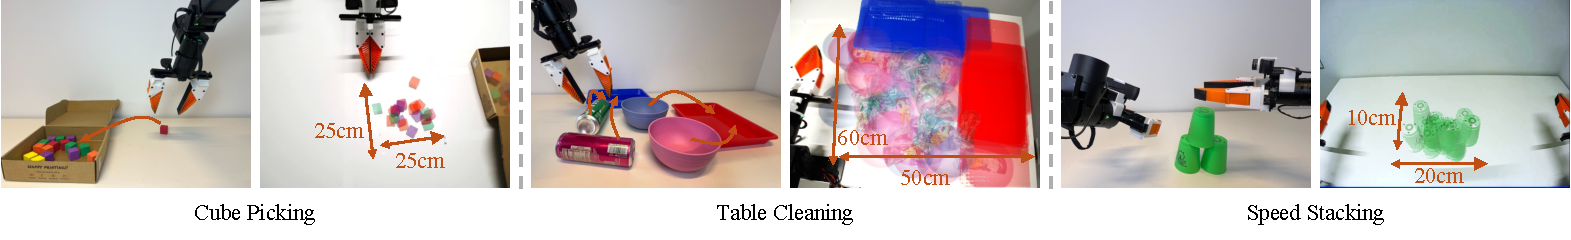
\includegraphics[width=1\linewidth]{images/real-world-task-setup.pdf}
%     \vspace{-15pt}
%     \caption{\textbf{Overview of the real-world tasks.} Task setups and corresponding object initialization distributions and workspace sizes for \pickcube, \cleantable, and \stackunstack.  These tasks vary in precision requirements, horizon length, and object interactions, highlighting the challenges of fast manipulation due to tight precision requirements, long task horizons, and complex object interactions.}
% \label{fig:real-world-setup}
% \vspace{-18pt}
% \end{figure*}


\begin{table*}[t]
  \centering
\vspace{-10pt}
    
  \fontsize{5.8pt}{6.8pt}\selectfont
  \renewcommand{\arraystretch}{0.92}
  \setlength{\tabcolsep}{1.2pt}

  \resizebox{\textwidth}{!}{
  \begin{tabular}{lc|cc|cc|cc||cc|cc|cc||ccc}
    \toprule
    Task & Metric
    & \multicolumn{6}{c||}{\textbf{Diffusion Policy}}
    & \multicolumn{6}{c||}{\textbf{Regression Policy}}
    & \multicolumn{3}{c}{\textbf{DemoSpeedUp Comparison}} \\
    \cmidrule(lr){3-8}
    \cmidrule(lr){9-14}
    \cmidrule(lr){15-17}

    & 
    & \multicolumn{2}{c|}{1X}
    & \multicolumn{2}{c|}{2X}
    & \multicolumn{2}{c||}{4X}
    & \multicolumn{2}{c|}{1X}
    & \multicolumn{2}{c|}{2X}
    & \multicolumn{2}{c||}{4X}
    & DemoSpeedUp
    & \makecell{Diff. +\\BSP 4X}
    & \makecell{Reg. +\\BSP 4X} \\
    \cmidrule(lr){3-4}
    \cmidrule(lr){5-6}
    \cmidrule(lr){7-8}
    \cmidrule(lr){9-10}
    \cmidrule(lr){11-12}
    \cmidrule(lr){13-14}

    & 
    & Diff.
    & \makecell{Diff. +\\BSP}
    & Diff.
    & \makecell{Diff. +\\BSP}
    & Diff.
    & \makecell{Diff. +\\BSP}
    & Reg.
    & \makecell{Reg. +\\BSP}
    & Reg.
    & \makecell{Reg. +\\BSP}
    & Reg.
    & \makecell{Reg. +\\BSP}
    & 
    & 
    & \\
    \midrule

    \makecell{Cube \\ Picking} & \cellMetric
    & \cellSRtime{19/20}{6.48s}
    & \cellSRtime{\greenNum{20/20}}{\purpleNum{6.31s}}
    & \cellSRtime{20/20}{4.58s}
    & \cellSRtime{\greenNum{20/20}}{\purpleNum{3.43s}}
    & \cellSRtime{20/20}{3.52s}
    & \cellSRtime{\greenNum{20/20}}{\purpleNum{2.45s}}
    & \cellSRtime{18/20}{9.84s}
    & \cellSRtime{\greenNum{19/20}}{\purpleNum{7.92s}}
    & \cellSRtime{15/20}{5.55s}
    & \cellSRtime{\greenNum{19/20}}{\purpleNum{3.36s}}
    & \cellSRtime{19/20}{3.74s}
    & \cellSRtime{\greenNum{19/20}}{\purpleNum{2.08s}}
    & \cellSRtime{18/20}{6.66s}
    & \cellSRtime{\greenNum{20/20}}{2.45s}
    & \cellSRtime{19/20}{\purpleNum{2.08s}} \\

    \midrule

    \makecell{Table \\ Cleaning} & \cellMetric
    & \cellSRtime{11/20}{41.40s}
    & \cellSRtime{\greenNum{15/20}}{\purpleNum{36.97s}}
    & \cellSRtime{\greenNum{15/20}}{28.87s}
    & \cellSRtime{14/20}{\purpleNum{20.81s}}
    & \cellSRtime{\greenNum{12/20}}{23.31s}
    & \cellSRtime{11/20}{\purpleNum{18.05s}}
    & \cellSRtime{13/20}{49.70s}
    & \cellSRtime{\greenNum{18/20}}{\purpleNum{38.47s}}
    & \cellSRtime{13/20}{34.48s}
    & \cellSRtime{\greenNum{18/20}}{\purpleNum{19.11s}}
    & \cellSRtime{13/20}{23.57s}
    & \cellSRtime{\greenNum{14/20}}{\purpleNum{11.80s}}
    & \cellSRtime{3/20}{49.47s}
    & \cellSRtime{11/20}{18.05s}
    & \cellSRtime{\greenNum{14/20}}{\purpleNum{11.80s}} \\

    \midrule

    \makecell{Speed \\ Stacking} & \cellMetric
    & \cellSRtime{14/20}{20.47s}
    & \cellSRtime{\greenNum{14/20}}{\purpleNum{18.13s}}
    & \cellSRtime{15/20}{13.66s}
    & \cellSRtime{\greenNum{15/20}}{\purpleNum{11.45s}}
    & \cellSRtime{\greenNum{9/20}}{10.49s}
    & \cellSRtime{7/20}{\purpleNum{9.62s}}
    & \cellSRtime{8/20}{19.75s}
    & \cellSRtime{\greenNum{16/20}}{\purpleNum{17.61s}}
    & \cellSRtime{4/20}{13.49s}
    & \cellSRtime{\greenNum{13/20}}{\purpleNum{10.98s}}
    & \cellSRtime{\greenNum{8/20}}{\purpleNum{10.42s}}
    & \cellSRtime{0/20}{NA}
    & \cellSRtime{3/20}{18.57s}
    & \cellSRtime{\greenNum{7/20}}{\purpleNum{9.62s}}
    & \cellSRtime{0/20}{NA} \\
    
    % \midrule

    % \makecell{Task 4} & \cellMetric
    % & \cellSRtime{x}{x}
    % & \cellSRtime{x}{x}
    % & \cellSRtime{x}{x}
    % & \cellSRtime{x}{x}
    % & \cellSRtime{x}{x}
    % & \cellSRtime{x}{x}
    % & \cellSRtime{x}{x}
    % & \cellSRtime{x}{x}
    % & \cellSRtime{x}{x}
    % & \cellSRtime{x}{x}
    % & \cellSRtime{x}{x}
    % & \cellSRtime{x}{x}
    % & \cellSRtime{x}{x}
    % & \cellSRtime{x}{x}
    % & \cellSRtime{x}{x} \\

    \bottomrule
  \end{tabular}
  }


  \caption{\textbf{Real-world quantitative results.}
  We report each method's success rate and average completion time on the real-world tasks.
  Completion time is averaged over successful rollouts. We highlight the results with higher success rates and shorter completion times in each comparison.}

  \vspace{-15pt}
  \label{tab:act-dp-results}
\end{table*}






\subsection{Real-world Results}
\vspace{-5pt}

Table~\ref{tab:act-dp-results} reports the overall success rates and average completion times. We organize our analysis around the following key findings.
\vspace{-5pt}

\textbf{Finding 1: BSP consistently shortens task completion time.} As highlighted in Tab.~\ref{tab:act-dp-results}, across all configurations, integrating BSP consistently reduces \textit{Avg. time}, regardless of whether it is paired with a Diffusion or Regression policy.
%
The efficiency of BSP acceleration is particularly pronounced in the long-horizon \cleantable task. Specifically, at a 4X speedup, integrating BSP with the Regression policy compresses the average completion time from $23.57\text{s}$ to $11.80\text{s}$ ($50\%$ reduction in duration), while simultaneously preserving task success rate ($13/20$ vs. $14/20$).



\textbf{Finding 2: BSP preserves task success, but aggressive speedup can exceed controller limits.}
\label{finding2}
%
BSP achieves faster execution while generally maintaining task success. Across diffusion and regression comparisons, BSP matches or improves success rate in 14 out of 18 settings.
%
This trend is particularly clear for the regression backbone: BSP improves the long-horizon Table Cleaning success from 13/20 to 18/20 at both $1\times$ and $2\times$ speedup, and improves Speed Stacking from 8/20 to 16/20 at $1\times$ speedup and from 4/20 to 13/20 at $2\times$ speedup.
\newline
At the same time, the results reveal a natural trade-off between execution speed and task robustness. 
% Especially under aggressive $4\times$ speedup, the baseline achieves higher success. 
%
For example, on \stackunstack, Regression+BSP outperforms the baselines at $1\times$ and $2\times$ speedup, but fails at $4\times$, achieving zero success because the aggressive BSP temporal scaling pushes the robot beyond the tracking limits of its low-level controller. 
% This suggests that more accurate and stiffer low-level controllers could further improve robustness at extreme speedups, which we leave as future work.



\begin{figure*}[t]
    \centering
    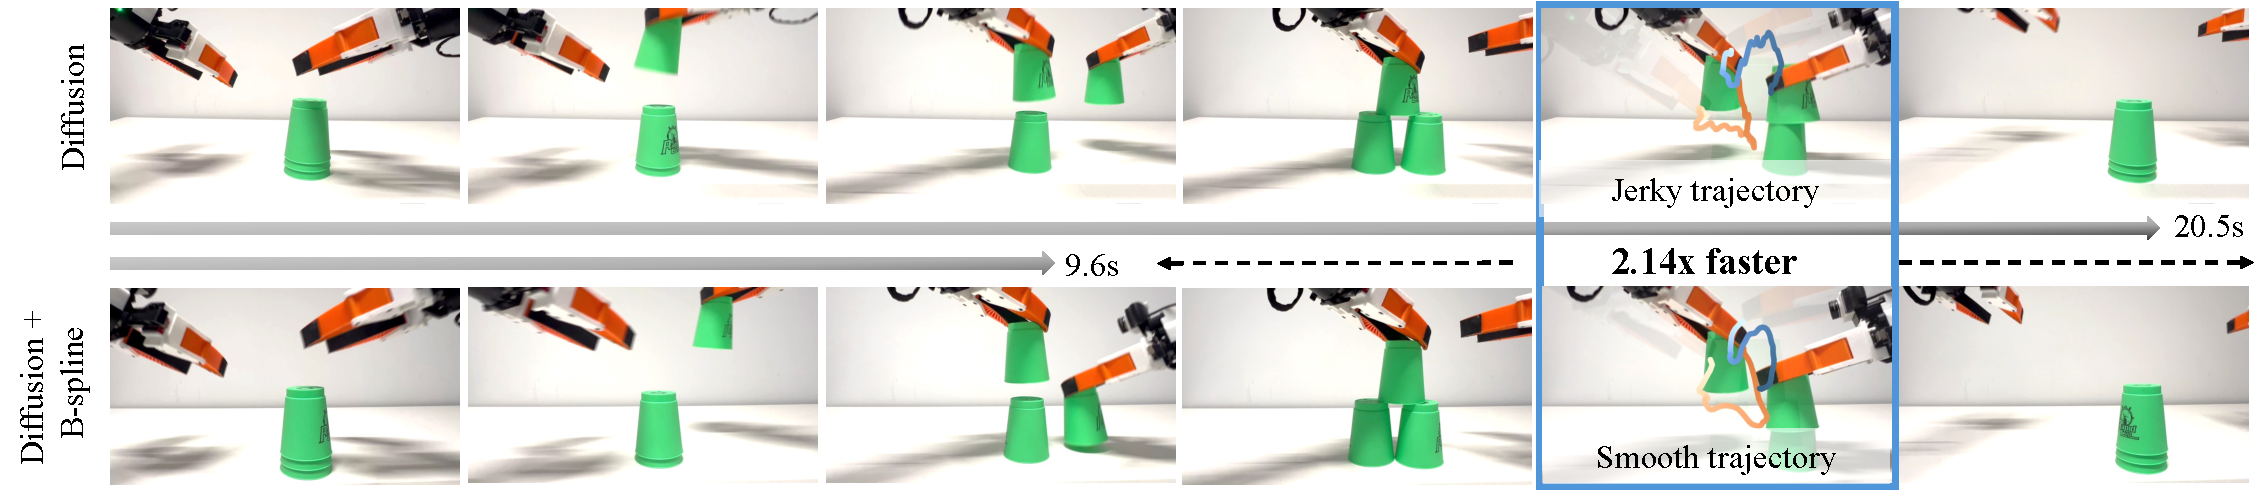
\includegraphics[width=1\linewidth]{images/smoothness-3.pdf}
\caption{\textbf{Real-world qualitative results.} We visualize key frames from the rollouts of \our and a diffusion policy on the speed stacking task, with the robot gripper tip trajectories overlaid on the frame, illustrating that \our achieves faster and smoother task execution.}
    \vspace{-15pt}

    \label{fig:qualitative-results}
\end{figure*}

\textbf{Finding 3: BSP produces smoother trajectories.}
%
During the experiments, we observed that \our produces substantially smoother executions than the baselines. We provide qualitative comparisons between \our and Diffusion Policy on the \stackunstack task in Fig.~\ref{fig:qualitative-results}, where we overlay the executed trajectories on video frames. \our yields smoother and faster motions, while the action chunks produced by Diffusion Policy often result in jerky executions due to discontinuities between consecutive chunks. Please visit \href{https://b-spline-policy.github.io/}{our website} for video results.



% For the DemoSpeedup baseline, temporal downsampling of demonstrations can skip critical intermediate states, especially when demonstrations are recorded at modest frequencies.
% This frequently produces jerky and unstable rollouts, leading to lower success rates and longer average completion times due to increased retries.
%

% Overall, \our achieves up to a \textbf{$4.21\times$} speedup over base imitation learning methods on the \cleantable task, while simultaneously achieving higher success rates.







\begin{wrapfigure}{r}{0.45\textwidth}
  \centering
  \vspace{-10pt}
  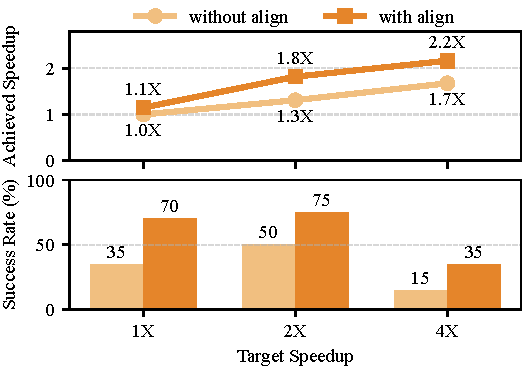
\includegraphics[width=\linewidth]{images/table5-combined-1.pdf}
    
  \caption{\textbf{Ablation study on inference-time segment alignment.}
  Aligning adjacent segments improves trajectory continuity, which becomes critical at high speeds, leading to higher success rates and more consistent realized speedups.}
  % Table5 in sheet2 google doc
  \label{fig:infer-align-success-speed}
  \vspace{-10pt}
\end{wrapfigure}




\textbf{Finding 4: Inference-time segment alignment is critical for BSP.}
%
Consistent with the smoother trajectories observed in Finding 3, we further find that trajectory continuity across consecutive spline segments is critical for stable high-speed execution. To better understand this, we conduct an ablation study on inference-time segment alignment on \stackunstack task. 
%
As shown in Fig.~\ref{fig:infer-align-success-speed}, segment alignment becomes increasingly important at higher execution speeds: when continuity is not enforced, success becomes highly sensitive to execution speed. From the policy perspective, such discontinuities effectively induce out-of-distribution (OOD) inputs, forcing the policy to spend additional steps replanning to return to the in-distribution regime, or causing outright task failure.





% \begin{wraptable}{r}{0.6\textwidth}
% \vspace{-1.0em}
% \centering
% \setlength{\tabcolsep}{5.0pt}
% \small
% \begin{tabular}{c|cccc}
% \toprule
% Method & Regression & BSP $1\times$ & BSP $2\times$ & BSP $4\times$ \\
% \midrule
% SPARC\;$\uparrow$ & $-8.01$ & $-5.89$ & $-5.28$ & $-5.11$ \\
% \bottomrule
% \end{tabular}
% \caption{\textbf{Quantitative results on smoothness.} 
% We report spectral arc length (SPARC) over successful episodes only. Higher is better; \our produces smoother trajectories.}
% \label{tab:smoothness}
% \vspace{-1.0em}
% \end{wraptable}

% \noindent\textbf{Low-level Controller.}
% An advantage of \our is that the B-spline representation provides velocity and acceleration at no extra cost via analytic derivatives. 
% We therefore implement a PD controller with feedforward terms, which can reduce tracking error~\cite{santibanez2001pd,an1986experimental,an1988model,an1987experimental}.
% Fig.~\ref{fig:ff-control} reports the corresponding success rates and completion times under different speedup rates. We found that \our better preserves success rates under aggressive speedup with a more accurate controller.
% %
% Since the policy is trained on teleoperated demonstrations collected with a standard PD controller, swapping to a more accurate controller can introduce a dynamics mismatch, leading to a noticeable performance drop at the original execution speed. 
% %
% As execution speed increases, the feedforward controller is able to better track velocity and acceleration and preserve success while achieving shorter completion times, indicating improved robustness under aggressive execution.


% \subsection{Discussion}
% \subsection{Limitations}
% \noindent\textbf{Limitations.}


% not sure if we need to add this
% \noindent\textbf{Relationship to post-hoc spline smoothing.}
% A natural simplified variant is to fit a B-spline online to each waypoint chunk predicted by a standard policy and then execute it with the same high-rate controller pipeline, and segment align scheme as \our.
% While this might speed up simple tasks, it remains limited by the waypoint representation: the policy still learns discrete samples at a fixed temporal resolution.
% In contrast, \our directly predicts a \emph{non-uniform} spline parameterization, allocating more knots to rapidly changing phases and fewer to smooth segments.
% Moreover, chunk-wise online fitting is inherently local, whereas fitting splines from full demonstrations can capture global structure during preprocessing, with more room for optimization.
% Empirically, \our improves success rates at the original speed on most tasks compared to the discrete action representation. We hypothesize that non-uniform knot placement contributes to this effect.




\vspace{-10pt}
\subsection{Simulation Benchmarks}
\vspace{-5pt}

For reproducibility, we also evaluate \our on simulated manipulation tasks to assess whether continuous B-spline action representations achieve performance comparable to standard action-chunking imitation learning methods on \textit{Push-T}~\cite{florence2022implicit,dp}, \textit{RoboMimic}~\cite{robomimic2021} and \textit{RoboCasa}~\cite{nasiriany2024robocasa}.

\begin{table*}[t]
  \centering
  \vspace{-6pt}

  \captionsetup[subtable]{
    justification=centering,
    singlelinecheck=false,
    font=footnotesize,
    skip=2pt
  }

  % ---------------- Left subtable (a) ----------------
  \begin{subtable}[t]{0.58\textwidth}
    \begin{minipage}[t][0.26\textheight][t]{\linewidth}
    \centering
    \fontsize{6.3pt}{7.3pt}\selectfont
    \renewcommand{\arraystretch}{0.92}
    \setlength{\tabcolsep}{2.0pt}

    \resizebox{\linewidth}{!}{
    \begin{tabular}{l|cccccc}
      \toprule
      Configuration 
      & PushT 
      & \makecell{Lift} 
      & \makecell{Turn off\\sink faucet} 
      & \makecell{Coffee\\press button} 
      & \makecell{Turn off\\microwave} 
      & \makecell{Close\\door} \\
      \midrule

      Diff. 1X Base  & 72\%            & 100\%             & 79\%            & 93\%            & 77\%            & 27\% \\
      Diff. 1X +BSP  & \greenNum{75\%} & \greenNum{100\%}  & \greenNum{85\%} & \greenNum{94\%} & \greenNum{89\%} & \greenNum{46\%} \\
      \midrule
      Reg. 1X Base   & 63\%            & \greenNum{99\%}   & 84\%            & 89\%            & 93\%            & 40\% \\
      Reg. 1X +BSP   & \greenNum{66\%} & 91\%              & \greenNum{94\%} & \greenNum{93\%} & \greenNum{97\%} & \greenNum{60\%} \\

      \bottomrule
    \end{tabular}
    }

    \caption{\textbf{Sim results.}}
    \label{tab:sim-results}
    \end{minipage}
  \end{subtable}
  \hfill
  % ---------------- Right subtable (b) ----------------
  \begin{subtable}[t]{0.39\textwidth}
    \begin{minipage}[t][0.26\textheight][t]{\linewidth}
    \centering
    \fontsize{5.8pt}{6.8pt}\selectfont
    \renewcommand{\arraystretch}{0.88}
    \setlength{\tabcolsep}{1.4pt}

    \resizebox{\linewidth}{!}{
    \begin{tabular}{c|cc|cc|cc}
      \toprule
      Metric
      & \multicolumn{6}{c}{\textbf{Diffusion Policy}} \\
      \cmidrule(lr){2-7}

      &
      \multicolumn{2}{c|}{1X}
      & \multicolumn{2}{c|}{2X}
      & \multicolumn{2}{c}{4X} \\
      \cmidrule(lr){2-3}
      \cmidrule(lr){4-5}
      \cmidrule(lr){6-7}

      &
      Diff.
      & \makecell{Diff. +\\BSP}
      & Diff.
      & \makecell{Diff. +\\BSP}
      & Diff.
      & \makecell{Diff. +\\BSP} \\
      \midrule

      \pushtcellMetric
      & \cellSRtime{0.47}{12.24s}
      & \cellSRtime{\greenNum{0.65}}{\purpleNum{7.20s}}
      & \cellSRtime{0.57}{9.22s}
      & \cellSRtime{\greenNum{0.71}}{\purpleNum{4.89s}}
      & \cellSRtime{0.59}{7.19s}
      & \cellSRtime{\greenNum{0.73}}{\purpleNum{2.87s}} \\

      \bottomrule
    \end{tabular}
    }

    \caption{\textbf{PushT-speedup results.}}
    \label{tab:pusht}
    \end{minipage}
  \end{subtable}

  \vspace{-90pt}
  \caption{\textbf{Simulation results.} In Table (a), we report average score on pushT and average success rate across other simulation benchmarks.
  In Table (b), we report the average score and average time for the PushT speedup.}
  \label{tab:combined-sim-real-results}
  \vspace{-10pt}
\end{table*}

\noindent\textbf{Quantitative performance.}
As shown in Table~\ref{tab:sim-results}, \our matches or outperforms the corresponding base policies across all evaluated tasks, except the RoboMimic Lift task.
%
% When paired with a diffusion decoder, \our achieves an average success rate of 76\%, while the regression-based variant attains an average success rate of 82\%.
On the more challenging RoboCasa tasks, \our consistently outperforms the baseline methods, demonstrating improved robustness in long-horizon manipulation scenarios.
Overall, these results indicate that representing actions as B-spline trajectories does not compromise imitation learning performance and can yield consistent gains over discrete-time action-chunking representations. 

\noindent\textbf{Acceleration in simulation.} Accelerating policies in simulation requires modifying the environment and low-level controllers to support the high-frequency execution required by BSP, which then requires re-collecting datasets, making it difficult to directly measure policy acceleration in each simulation benchmark. Therefore, we conduct this study on Push-T, a representative task that is easy to modify.
%
We collect 100 demonstrations in the PushT-speedup environment at 200 Hz. BSP is trained directly on the 200 Hz trajectories, while the diffusion policy baseline is trained on 10 Hz trajectories downsampled from the same data.
%
For each checkpoint, we evaluate 50 rollouts and report the average score. We define a rollout as successful if its score exceeds 0.9, which indicates near-complete coverage. For each successful rollout, we record the first time step at which the score exceeds 0.9, and report the average of this time across successful rollouts. For each setting, we evaluate the best three checkpoints and report the mean of these metrics.\newline 
%
As shown in Table~\ref{tab:pusht}, BSP consistently improves both the average score and completion time across all target speedups. The gains become pronounced at higher speedups: at $4\times$, Diff.+BSP achieves a higher average score ($0.73$ vs. $0.59$) while reducing completion time by more than half ($7.19$s to $2.87$s). This is because faster execution enables the Push-T agent to perform more corrective pushes within the maximum rollout time, leading to higher final coverage scores. 
%
% These results suggest that BSP not only accelerates execution but also improves task performance by enabling more retries and corrections within a fixed time budget.

% \begin{figure*}[t]
%   \centering
%   % --- Row 1: simulation tasks (full width) ---
%   % \includegraphics[width=0.98\textwidth]{images/sim-env.pdf}

%   \vspace{-4pt}

%   % --- Row 2: simulation results (two half-width figures) ---
%   % \includegraphics[width=0.98\textwidth]{images/sim-results.pdf}\hfill
%   \includegraphics[width=0.98\textwidth]{images/sim-tasks-and-results.pdf}\hfill
%   % \includegraphics[width=0.48\textwidth]{images/sim-results-dp.pdf}
%     \vspace{-5pt}
%       \caption{\textbf{Simulation benchmark tasks and results.} [Top row]: We evaluate seven simulation benchmark tasks in Push-T, RoboMimic, and RoboCasa. 
%   [Bottom row]: We report success rates of action-chunk policies and the B-spline policies, averaged over the three best checkpoints during training, evaluated 50 rollouts per task.}

%   \vspace{-10pt}
%   \label{fig:sim_results_act_dp}
% \end{figure*}
\vspace{-10pt}
\section{Limitations}
\vspace{-10pt}
\paragraph{Hardware Constraints and Policy Acceleration Limits.} As detailed in Section~\ref{finding2}, aggressively accelerating the policy introduces a drop in robustness; specifically, the Speed Stacking task drops to a 0\% success rate under a 4x speedup. 
%
This failure is primarily driven by the physical constraints of the low-cost robotic arms used in our experiments, whose low-level controllers lack the stiffness and accuracy required to track rapid action commands. We believe that integrating improved low-level controllers would significantly improve tracking robustness at extreme speeds, which we plan to explore in future work.

\vspace{-10pt}
\section{Conclusion}
\vspace{-10pt}
We propose \our, a novel action representation that parameterizes the actions as continuous curves using B-splines. \our improves trajectory smoothness and enables faster task completion with robust success rate.
%
To ensure stability during high-speed execution, we propose an inference-time segment alignment mechanism that effectively mitigates boundary discontinuities between successive spline segments.
%
Extensive empirical evaluations across diverse simulated and real-world manipulation tasks demonstrate that BSP significantly reduces task completion times, while consistently preserving or enhancing success rates over standard baselines.